% Math of Social Choice
% Oberlin College
% Isaac Hollander McCreery

\documentclass[mathserif,serif]{beamer}

\newcommand{\honor}{We affirm that we have adhered to the honor code on this assignment.}

% Another example tex file
% Oberlin College
% Isaac Hollander McCreery

% document information
\title[$n$-D Stable Matching]{Stable Jazz Ensembles: $n$-D Matching Problems}
\author[Brodner, Fogg, McCreery]{Simone Brodner \and Peter Fogg \and Isaac Hollander McCreery}
\date{May 5, 2014}

% packages
\usepackage[parfill]{parskip} % begin paragraphs with an empty line rather than an indent
%\usepackage{fullpage} % use more of the page
\usepackage{amsmath,amssymb,amsthm} % math stuff
\usepackage{paralist}
\usepackage{algorithm}
\usepackage[noend]{algorithmic}
\usepackage{moreenum}
\usepackage{graphicx}
\usepackage{ulem}

\AtBeginSection[]
{
	\begin{frame}
		\tableofcontents[currentsection]
	\end{frame}
}

\AtBeginSubsection[]
{
	\begin{frame}
		\tableofcontents[currentsection,currentsubsection]
	\end{frame}
}

%% formatting pages, etc.
%\renewcommand{\baselinestretch}{1.1}
%\setlength{\headheight}{15.2pt}
%\setlength{\headsep}{15pt}
%\setlength{\textheight}{592pt}
%\setlength{\footskip}{30pt}
%\renewcommand{\headrulewidth}{0pt}
%\renewcommand{\footrulewidth}{0pt}

%% format the header
%\fancyhf{}
%\lhead{\student}
%\rhead{\today}
%\cfoot{\thepage}
%\pagestyle{fancy}
%
%% format the title
%\renewcommand\maketitle{
%\begin{center}
%	\textsc{\Large \name: Homework \#\hwk} \\ [12pt]
%	\textsc{\student}
%\end{center}
%}

%% list formatting
%\renewcommand{\theenumi}{\arabic{enumi}.}
%\renewcommand{\labelenumi}{\theenumi}
%\renewcommand{\theenumiii}{\roman{enumiii}.}
%\renewcommand{\labelenumiii}{\theenumiii}
%\renewcommand{\theenumiv}{\greek{enumiv})}
%\renewcommand{\labelenumiv}{\theenumiv}
%
%%%
%% The following are definitions so that you can use numbered lemmas, claims, etc.
%%%
%\newtheorem{lemma}{Lemma}
%\newtheorem*{lem}{Lemma}
%\newtheorem{definition}{Definition}
%\newtheorem{notation}{Notation}
%\newtheorem*{claim}{Claim}
%\newtheorem*{fclaim}{False Claim}
%\newtheorem{observation}{Observation}
%\newtheorem{conjecture}[lemma]{Conjecture}
%\newtheorem{theorem}[lemma]{Theorem}
%\newtheorem{corollary}[lemma]{Corollary}
%\newtheorem{proposition}[lemma]{Proposition}
%\newtheorem*{rt}{Running Time}

\newcommand{\upth}{^{\text{th}}}
\newcommand{\eval}{\Big|}
\newcommand{\NP}{NP}


\begin{document}

\frame{\titlepage}

\begin{frame}
	\tableofcontents
\end{frame}

% BEGIN Ike

\section{3GSM \& 3PSA}

\begin{frame}
	\frametitle{3GSM: 3-gender stable marriage problem}

	$n$ alto sax players, $n$ bassists, $n$ drummers, each ranks some of the $n(n-1)$ possible pairs to make an
	ensemble of one alto player, one bassist, and one drummer.
	May rank some and keep the rest as unacceptable.
	Stability is reached when
	\[
	\not\exists \: a \in A, b \in B, d \in D
	\]
	such that
	\[
	(b,d) >_a \mu(a) \text{ and } (a,d) >_b \mu(b) \text{ and } (a,b) >_d \mu(d).
	\]
	Can we guarantee a solution, and can we find an algorithm to compute a stable marriage?
\end{frame}

\begin{frame}
	\frametitle{3PSA: 3-person stable assignment problem}

	$3n$ people, each ranks some of the $\frac{1}{2}(3n-1)(3n-2)$ possible pairs of other students.
	May rank some and keep the rest as unacceptable.
	Stability is reached if
	\[
	\not\exists \: p, q, r \in P
	\]
	such that
	\[
	(q,r) >_p \mu(p) \text{ and } (p,r) >_q \mu(q) \text{ and } (p,q) >_r \mu(r).
	\]

	We probably can't guarantee a solution, but can we find an algorithm to decide?
\end{frame}

\begin{frame}
	\frametitle{Motivations}

	
\includegraphics[width=\textwidth]{cat-jazz}
        \footnote{https://home.oberlin.edu/home/2013/03/29/jazz-at-the-cat}
\end{frame}

\begin{frame}
	\frametitle{Motivations}

	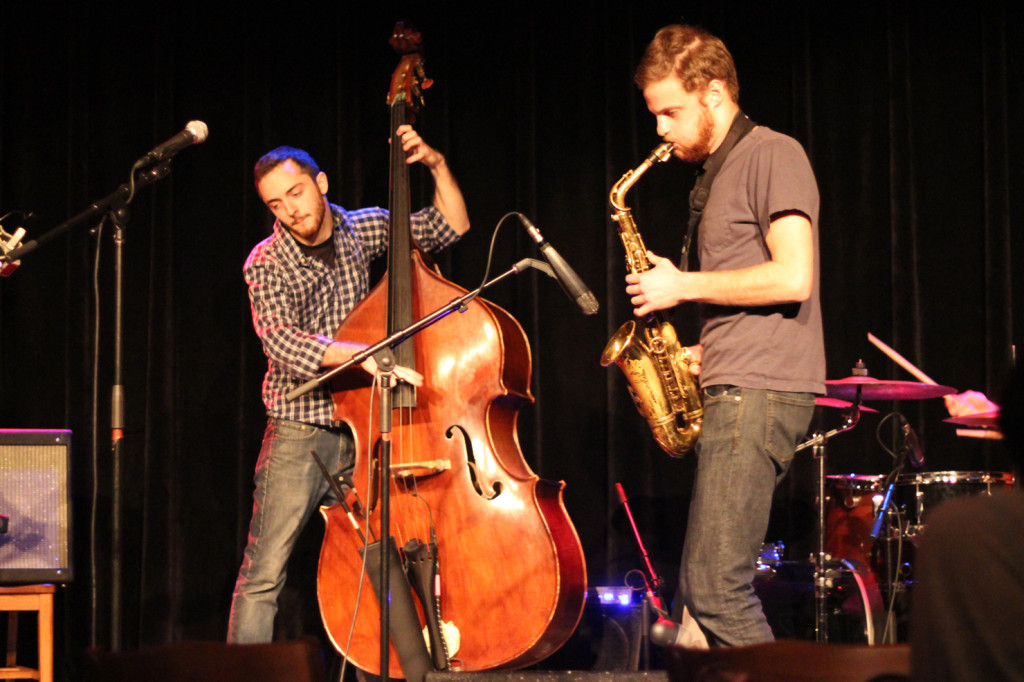
\includegraphics[width=\textwidth]{mwsb-jazz}
        \footnote{http://oberlinreview.org/wp-content/uploads/2013/12/MenShortBeards\_by-Yvette-Chen\_MASTERWEB-1024x682.jpg}
\end{frame}

% END Ike

% BEGIN Peter

\begin{frame}
  \frametitle{Existence of Stable Matchings}

    \begin{center}
      \begin{tabular}{c | c c c c}
        $\alpha_1$ & $\beta_1\delta_2$ $\beta_1\delta_1$ $\beta_2\delta_2$ $\beta_2\delta_1$ \\
        $\alpha_1$ & $\beta_2\delta_2$ $\beta_1\delta_1$ $\beta_2\delta_1$ $\beta_1\delta_2$ \\ \hline
        $\beta_1$ & $\alpha_2\delta_1$ $\alpha_1\delta_2$ $\alpha_1\delta_1$ $\alpha_2\delta_2$ \\
        $\beta_2$ & $\alpha_2\delta_1$ $\alpha_1\delta_1$ $\alpha_2\delta_2$ $\alpha_1\delta_2$ \\ \hline
        $\delta_1$ & $\alpha_1\beta_2$ $\alpha_1\beta_1$ $\alpha_2\beta_1$ $\alpha_2\beta_2$ \\
        $\delta_2$ & $\alpha_1\beta_1$ $\alpha_2\beta_2$ $\alpha_1\beta_2$ $\alpha_2\beta_1$ \\
      \end{tabular}
      \begin{tabular}{c | c}
        Marriage & Destabilized by \\ \hline
        $\{\alpha_1, \beta_1, \delta_1\}, \{\alpha_2, \beta_2, \delta_2\}$ & $\alpha_1\beta_1\delta_2$ \\
        $\{\alpha_1, \beta_1, \delta_2\}, \{\alpha_2, \beta_2, \delta_1\}$ & $\alpha_2\beta_1\delta_1$ \\
        $\{\alpha_1, \beta_2, \delta_1\}, \{\alpha_2, \beta_1, \delta_2\}$ & $\alpha_1\beta_1\delta_2$ \\
        $\{\alpha_1, \beta_2, \delta_2\}, \{\alpha_2, \beta_1, \delta_1\}$ & $\alpha_2\beta_2\delta_2$ \\
      \end{tabular}
    \end{center}
\end{frame}

\section{\NP-Completeness}

\begin{frame}
  \frametitle{NP-Completeness}
  \begin{itemize}
  \item A problem is in P if it can be solved efficiently
  \item Searching, sorting, parsing, finding 2D stable matchings, etc.
  \item In NP if a potential solution can be checked efficiently
  \item NP-hard if at least as hard as all problems in NP
  \item NP-complete if NP-hard \emph{and} in NP
  \item Traveling salesman, $k$-coloring, etc.
  \end{itemize}
\end{frame}

\begin{frame}
  \frametitle{NP-Completeness}
  \begin{itemize}
  \item To show a problem is  NP-complete, we use it to solve another NP-hard problem
  \item Example: Vertex Cover (VC) and Independent Set (IS)
    \begin{itemize}
    \item VC: Given a graph $G = (V, E)$ and $k \in \mathbb{N}$, select $k$ vertices s.t. all edges have at least one endpoint covered
    \item IS: Given a graph $G$ and $k \in \mathbb{N}$, find $k$ vertices s.t. no two vertices share an edge
    \item Given a solution $S$ of one problem, we can convert to the other by taking the complement of $S$ with respect to $V$
    \item VC and IS are equally hard!
    \end{itemize}
  \item NP-hard problems are thought to be impossible to solve efficiently (but we're not sure yet)
  \end{itemize}
\end{frame}

% END Peter

% BEGIN Ike

\section{3GSM is \NP-Complete}

\subsection{Setup}

\begin{frame}
	\frametitle{3DM: 3-dimensional matching problem}

	Three sets $A'$, $B'$, and $D'$ of size $n$ and $T' \subseteq A' \times B' \times D'$.  Is there a complete
	matching $M' \subseteq T'$?

	Simplifying assumption: no element of $A'$, $B'$, or $D'$ appears in more than three triples of $T'$; still
	\NP-Complete. \footnote{Garey \& Johnson. \textit{Computer and Intractability: a guide to the theory of NP-completeness,} W.H. Freeman \& Co., NY, 1979.}
\end{frame}

\begin{frame}
	\frametitle{Setup}

	Suppose $A' = \{a_1, a_2, \dots, a_n\}$, $B' = \{b_1, b_2, \dots, b_n\}$, $D' = \{d_1, d_2, \dots, d_n\}$.  No
	$a_i \in A'$ appears in more than 3 triples of $T'$.

	Create sets $A, B, D$ each of size $3n$:
	\begin{align*}
	A &= \bigcup_{a_i \in A'} \{a_i[1], a_i[2], a_i[3]\} \\
	B &= B' \cup \bigcup_{a_i \in A'} \{w_{a_i}, y_{a_i}\} \\
	D &= D' \cup \bigcup_{a_i \in A'} \{x_{a_i}, z_{a_i}\}.
	\end{align*}
\end{frame}

\begin{frame}
	\frametitle{Preferences}

	\begin{tabular}{r | c c c}
		\vdots \\
		$a_i[1]$ &	$w_{a_i}x_{a_i}$ &	$y_{a_i}z_{a_i}$ &	$b_{j_1}d_{l_1}$ \\
		$a_i[2]$ &	$w_{a_i}x_{a_i}$ &	$y_{a_i}z_{a_i}$ &	$b_{j_2}d_{l_2}$ \\
		$a_i[3]$ &	$w_{a_i}x_{a_i}$ &	$y_{a_i}z_{a_i}$ &	$b_{j_3}d_{l_3}$ \\
		\vdots \\
		\hline
		\vdots \\
		$b_i$ &		\dots \\
		$w_{a_i}$ &	$a_i[1]x_{a_i}$ &	$a_i[2]x_{a_i}$ &	$a_i[3]x_{a_i}$ \\
		$y_{a_i}$ &	$a_i[1]x_{a_i}$ &	$a_i[2]x_{a_i}$ &	$a_i[3]x_{a_i}$ \\
		\vdots \\
		\hline
		\vdots \\
		$d_i$ &		\dots \\
		$x_{a_i}$ &	$a_i[3]w_{a_i}$ &	$a_i[2]w_{a_i}$ &	$a_i[1]w_{a_i}$ \\
		$z_{a_i}$ &	$a_i[3]y_{a_i}$ &	$a_i[2]y_{a_i}$ &	$a_i[1]y_{a_i}$ \\
		\vdots \\
	\end{tabular}
\end{frame}

\begin{frame}
	\frametitle{A lemma}

	\emph{Lemma.}
	Every $w_{a_i}$, $y_{a_i}$, $x_{a_i}$, and $z_{a_i}$ must be matched.

	\emph{Proof.}
	Unless $x_{a_i}$ is matched, $a_i[1]w_{a_i}x_{a_i}$ is destabilizing, and $x_{a_i}$ must be matched with
	$w_{a_i}$.

	Similarly, unless $z_{a_i}$ is matched, $a_i[1]y_{a_i}z_{a_i}$ or $a_i[2]y_{a_i}z_{a_i}$ is destabilizing, and
	$z_{a_i}$ must be matched with $y_{a_i}$.
	\qed
\end{frame}

% END Ike

% BEGIN Peter

\subsection{3GSM is \NP-Complete}

\begin{frame}
  \frametitle{NP-Completeness of 3GSM}
  \textbf{Theorem 1.} If $T'$ contains a matching $M'$, the 3GSM instance has a stable marriage $M$.

  \textit{Proof.} For each $a_i \in A'$, one of $a_ib_{j_1}d_{l_1}, a_ib_{j_2}d_{l_2}, a_ib_{j_3}d_{l_3}$ are in $M'$. We add to $M$
  \begin{align*}
    \begin{cases}
      a_i[1]b_{j_1}d_{l_1}, a_i[2]w_{a_i}x_{a_i}, a_i[3]y_{a_i}z_{a_i} & \text{if } a_ib{j_1}d_{l_1} \in M' \\
      a_i[1]w_{a_i}x_{a_i}, a_i[2]b_{j_2}d_{l_2}, a_i[3]y_{a_i}z_{a_i} & \text{if } a_ib{j_2}d_{l_2} \in M' \\
      a_i[1]w_{a_i}x_{a_i}, a_i[2]y_{a_i}z_{a_i}, a_i[3]b_{j_3}d_{l_3} & \text{if } a_ib{j_3}d_{l_3} \in M'. \\
    \end{cases}
  \end{align*}
  $M'$ is complete, so this is a marriage. Furthermore, it is stable -- no element of $A$ is a member of a destabilizing triple. The only pairs which can form such a triple are $w_{a_i}x_{a_i}$ and $y_{a_i}z_{a_i}$, but the $w_{a_i}$'s matches are one of their top choices, and the $x_{a_i}$'s preference is in exactly reversed order (similarly for $y_{a_i}$ and $z_{a_i}$).
\end{frame}

\begin{frame}
  \frametitle{NP-Completeness of 3GSM}
  \textbf{Theorem 2.} If our 3GSM instance has a stable marriage $M$, $T'$ contains a complete matching.

  \textit{Proof.} By our lemma, for each $a_i$, two of its clones are matched with $w_{a_i}x_{a_i}$ and $y_{a_i}z_{a_i}$. Call $M'$ the remaining elements. $M'$ is a matching, since it is a subset of the marriage $M$.

  By the construction of $I$, each $a_i$ is matched with some pair in $T'$, making $M'$ a complete matching of $T'$.
\end{frame}

\begin{frame}
  \frametitle{NP-Completeness of 3GSM}
  \textbf{Theorem 3.} 3GSM is NP-complete.

  \textit{Proof.} We have shown that we have a solution to 3DM iff we have a solution to the corresponding instance to 3GSM. Furthermore, we can efficiently check that a marriage is stable, and so 3GSM $\in$ NP.
\end{frame}

% END Peter

% BEGIN Simone

\subsection{Extension to 3PSA}

\begin{frame}
	\frametitle{Extending 3GSM to 3PSA}

	3GSM: $k$ disjoint triples from 3 disjoint sets of size $k$ \\
	3PSA: $k$ disjoint triples from 1 set of size $3k$\\
	\newline
	Given 3GSM setup and solution, construct a 3PSA setup and solution: \\
		$S = A \cup B \cup D$\\
		$\forall s \in S$ give the same preferences as in 3GSM.\\

	%	What's missing?\\
	%		- Pairs where both elements in the same original set (i.e. $\{ a_1, a_2 \}$) \\
	%		- Pairs not ranked in original 3GSM (we said incomplete was ok)\\
\end{frame}

\begin{frame}
	\frametitle{3PSA is NP-Complete} 
		Matching we found in 3GSM is also a solution in this constructed 3PSA \\
		\newline
		\emph{Claim.} 3PSA also NP-Complete\\
		\emph{Proof.} Any stable assignment in this instance involves only inherited items and is
	therefore also a marriage in 3GSM instance: \\
			- Suppose there were elements $a_i \in A, b_j \in B, d_l \in D$ not matched to inherited items;\\
			then $a_i b_j d_l$ would be a destabilizing triple\\ %because it is ranked ahead of whatever other matching? still true with incomplete?
			- This would also be a destabilizing triple in 3GSM (only inherited items);\\
			so, a solution in this 3PSA instance is also a solution in the 3GSM instance. \\

\end{frame}

\section{Wrap up}

\begin{frame}

	\frametitle{Conclusions}
	
	
\includegraphics[width=\textwidth]{us}
	
\end{frame}

\begin{frame}

	\frametitle{Open Questions}

	\emph{Consistency.} Within these proofs, preferences are allowed to be ``inconsistent:" for some $a \in A$, they may not consistently rank pairs with $\beta_1$ over pairs with $\beta_2$--the ordering may completely depend on the other element in the pair. \\

		\begin{itemize}Does this ``make sense"/seem reasonable?\\ 
			\item Jazz Trios? -- sure, maybe\\
			\item Foods? -- definitely (chocolate \& peanut butter: good, chocolate \& refried beans: bad)\\
			\item Groups for class? -- Not as much (want to work with your best friend \& anyone else more than any two acquaintances)\\
		\end{itemize}
	\newline
	Is this problem still NP-Hard if we assert consistency?
	\newline
\end{frame}
\begin{frame}
	\frametitle{Open Questions}
	\emph{Consistency.} Rather than ranking pairs, have $A$ rank $B$, $B$ rank $C$, $C$ rank $A$.  \\
	Destabilizing triple is then: $abd \notin M$ where $a b_1 d_1, a_2 b d_2, a_3 b_3 d \in M$ and $b \geq_a b_1, d \geq_b d_2, a \geq_d a_3$.\\

	Are there situations where this makes more sense?\\ % THINK OF SOME
	Is this problem easier?

\end{frame}


\begin{frame}
	\honor
\end{frame}

% END Simone

\end{document}
